\documentclass[12pt]{article}
\usepackage[utf8]{inputenc}
\usepackage{amsmath}

\title{ECE 3413 Lab 02\\*Polynomials and Transfer Functions}
\author{Leomar Dur\'an}
\date{$9^{\text{th}}$ February 2023}

\usepackage{siunitx}

\usepackage{titling}
\usepackage{standalone}
\usepackage{pdfpages}
\usepackage{minted}

\usepackage{matlab}
% \newcommand*\matlabtitle\subsection
% \newcommand*\matlabheading\subsubsection
% \newcommand*\mlcell[1]{#1}
% \newenvironment{matlaboutput}{%
    % \minted{matlab}%
% }%
% {%
    % \endminted%
% }%
% \newenvironment{matlabtableoutput}{}{}%

\usepackage{mathtools}%
\DeclarePairedDelimiter\brao()%
\DeclarePairedDelimiter\brac[]%
\DeclarePairedDelimiter\braco[)%
\DeclarePairedDelimiter\Brac\{\}%
\DeclarePairedDelimiter\norm\lVert\rVert%
\DeclarePairedDelimiter\piecefn\{.
\DeclarePairedDelimiter\evalat.|

% save original spacing between paragraphs
\newlength\oldparskip
\setlength\oldparskip\parskip
% save new space between paragraphs
\newlength\newparskip
\setlength\newparskip\baselineskip
% commands for set/reset
\newcommand*\setparskip{\setlength\parskip\newparskip}
\newcommand*\resetparskip{\setlength\parskip\oldparskip}
% apply new space
\setparskip
% no indent
\setlength\parindent{0pt}

\def\hr{{\par\noindent\rule{\textwidth}{0.4pt}}}

\begin{document}

\maketitle
\newpage

\section{Introduction}

The purpose of this experiment is to reinforce and build on the introduction to Matlab from Lab 01.

This lab reviews operations on polynomials and teaches how to work with transfer functions.

In this example,
along with converting between the sum and factored forms of polynomials,
we will also experiment with converting between various forms of the transfer function,
namely ratio of polynomials, zero/pole/gain form and the time-domain form.

\section{Procedure}

\subsection{Parts 1.1, 1.2 -- Roots and polynomial forms}

We revisit the use of the representation of polynomials using row vectors of coefficients from highest to lowest order, 
as well as the use of \mintinline{matlab}{poly} to convert roots to the polynomials with those roots and
\mintinline{matlab}{roots} to convert polynomials to their roots.

\subsection{Part 1.3 -- Ratio of polynomials and zero/pole/gain forms}

We revisit the \mintinline{matlab}{tf} function that creates a transfer function as a ratio of polynomials and formally introduce the \mintinline{matlab}{zpk} mentioned in Lab 01. This latter function creates a transfer function as a vector of zeroes, a vector of poles, and the gain.

\subsubsection{Conversion between transfer function forms}

In addition to creating transfer functions from vectors, 
\mintinline{matlab}{tf} and \mintinline{matlab}{zpk} can be used to convert back and forth between the different forms of transfer functions.

\subsection{Part 1.4 -- Partial fraction expansion}

\subsubsection{Storing transfer functions}

To store transfer functions,
I chose to store them each as a numerator and denominator, storing 2 factors, each potentially as trinomials.
The factors are then multiplied.

I could have used the ZPK model, but this would have required a separate vector for the gains.

Now when a polynomial with $S + 1$ terms is multiplied with a polynomial with $T + 1$ terms, the resulting vector will be of length $S + T + 1$,

Now if we multiply together $2$ polynomials all with $S + 1$ terms,
we will have a product polynomial with $2S + 1$ terms,
and $3$ polynomials this is the same as a polynomial with $2S + 1$ terms and a polynomial of $S + 1$ terms, which
will give $\brao*{2S} + \brao*{S} + 1 = 3S + 1$ terms.
Thus, multiplying $P + 1$ polynomials with $S + 1$ terms will produce a polynomial with $\brao*{P + 1}S + 1$ terms.

Let $Q := P + 1$ and $T = S + 1$, then multiplying $Q$ polynomials all with $T$ terms each will produce a polynomial of $Q\brao*{T - 1} + 1$ terms. Thus, we can store the numerator and denominator of each polynomial in $2\brao*{3 - 1} + 1 = 5$ terms.

\subsubsection{Partial fraction decomposition in Matlab}

Matlab provides the \mintinline{matlab}{residue} function which returns a vector of 

\section{Results}

\hr
\resetparskip
% This LaTeX was auto-generated from MATLAB code.
% To make changes, update the MATLAB code and export to LaTeX again.

\documentclass{article}

\usepackage[utf8]{inputenc}
\usepackage[T1]{fontenc}
\usepackage{lmodern}
\usepackage{graphicx}
\usepackage{color}
\usepackage{hyperref}
\usepackage{amsmath}
\usepackage{amsfonts}
\usepackage{epstopdf}
\usepackage[table]{xcolor}
\usepackage{matlab}

\sloppy
\epstopdfsetup{outdir=./}
\graphicspath{ {./part01_poles_zeros_mlx_images/} }

\begin{document}

\matlabtitle{Part 1 $-$ Poles and zeros}


\matlabheading{1ab. Roots}

\begin{par}
\begin{flushleft}
Calculate the roots of each of the following polynomials
\end{flushleft}
\end{par}

\begin{matlabsymbolicoutput}
\hskip1em $\displaystyle P_1 =s^6 +s^5 +2\,s^4 +8\,s^3 +7\,s^2 +15\,s+12$
\hskip1em $\displaystyle P_2 =s^6 +s^5 +4\,s^4 +3\,s^3 +7\,s^2 +15\,s+18$
\end{matlabsymbolicoutput}


\begin{par}
\begin{flushleft}
The roots for each polynomial are
\end{flushleft}
\end{par}

\begin{matlabtableoutput}
{
\begin{tabular} {|c|c|c|c|}\hline
\mlcell{ } & \mlcell{CartesianForm} & \mlcell{r} & \mlcell{thetaDeg} \\ \hline
\mlcell{1} & \mlcell{0.9979 + 1.6070i} & \mlcell{1.8916} & \mlcell{58.1624} \\ \hline
\mlcell{2} & \mlcell{0.9979 - 1.6070i} & \mlcell{1.8916} & \mlcell{301.8376} \\ \hline
\mlcell{3} & \mlcell{-1.8615 + 0.0000i} & \mlcell{1.8615} & \mlcell{180} \\ \hline
\mlcell{4} & \mlcell{-0.1302 + 1.4299i} & \mlcell{1.4358} & \mlcell{95.2009} \\ \hline
\mlcell{5} & \mlcell{-0.1302 - 1.4299i} & \mlcell{1.4358} & \mlcell{264.7991} \\ \hline
\mlcell{6} & \mlcell{-0.8739 + 0.0000i} & \mlcell{0.8739} & \mlcell{180} \\ 
\hline
\end{tabular}
}
\end{matlabtableoutput}
\begin{matlabtableoutput}
{
\begin{tabular} {|c|c|c|c|}\hline
\mlcell{ } & \mlcell{CartesianForm} & \mlcell{r} & \mlcell{thetaDeg} \\ \hline
\mlcell{1} & \mlcell{1.0375 + 1.3227i} & \mlcell{1.6811} & \mlcell{51.8922} \\ \hline
\mlcell{2} & \mlcell{1.0375 - 1.3227i} & \mlcell{1.6811} & \mlcell{308.1078} \\ \hline
\mlcell{3} & \mlcell{-0.4632 + 1.9333i} & \mlcell{1.9880} & \mlcell{103.4723} \\ \hline
\mlcell{4} & \mlcell{-0.4632 - 1.9333i} & \mlcell{1.9880} & \mlcell{256.5277} \\ \hline
\mlcell{5} & \mlcell{-1.0743 + 0.6764i} & \mlcell{1.2695} & \mlcell{147.8047} \\ \hline
\mlcell{6} & \mlcell{-1.0743 - 0.6764i} & \mlcell{1.2695} & \mlcell{212.1953} \\ 
\hline
\end{tabular}
}
\end{matlabtableoutput}

\matlabheading{2. Polynomial form}

\begin{par}
\begin{flushleft}
Calculate the polynomial form and roots of
\end{flushleft}
\end{par}

\begin{matlabsymbolicoutput}
\hskip1em $\displaystyle P_3 ={\left(s-1\right)}\,{\left(s-2\right)}\,{\left(s+2\right)}\,{\left(s+3\right)}\,{\left(s+4\right)}\,{\left(s+5\right)}$
\end{matlabsymbolicoutput}

\begin{par}
\begin{flushleft}
The polynomial form is
\end{flushleft}
\end{par}

\begin{matlabsymbolicoutput}
P3\_s = 

\hskip1em $\displaystyle s^6 +11\,s^5 +31\,s^4 -31\,s^3 -200\,s^2 -52\,s+240$
\end{matlabsymbolicoutput}

\begin{par}
\begin{flushleft}
The roots of the polynomial are
\end{flushleft}
\end{par}

\begin{matlaboutput}
P3_roots = 6x1    
   -5.0000
   -4.0000
   -3.0000
   -2.0000
    2.0000
    1.0000

\end{matlaboutput}

\matlabheading{3a. Converting to polynomial numerator and denominator.}

\begin{par}
\begin{flushleft}
Represent
\end{flushleft}
\end{par}

\begin{matlaboutput}
G1 =
 
  9 (s+2) (s+3) (s+8) (s-6)
  --------------------------
  s (s+7) (s+10) (s-3) (s-2)
 
Continuous-time zero/pole/gain model.
\end{matlaboutput}

\begin{par}
\begin{flushleft}
using polynomials in the numerator and denominator.
\end{flushleft}
\end{par}

\begin{par}
\begin{flushleft}
In polynomial numerator and denominator, the transfer function
\end{flushleft}
\end{par}

\begin{matlaboutput}
G1_tf =
 
  9 s^4 + 63 s^3 - 288 s^2 - 2052 s - 2592
  ----------------------------------------
   s^5 + 12 s^4 - 9 s^3 - 248 s^2 + 420 s
 
Continuous-time transfer function.
\end{matlaboutput}

\matlabheading{3b. Converting to zero-pole-gain form.}

\begin{par}
\begin{flushleft}
Represent 
\end{flushleft}
\end{par}

\begin{matlaboutput}
G2 =
 
         s^4 + 17 s^3 + 99 s^2 + 223 s + 140
  -------------------------------------------------
  s^5 + 32 s^4 + 363 s^3 + 2092 s^2 + 5052 s + 4320
 
Continuous-time transfer function.
\end{matlaboutput}

\begin{par}
\begin{flushleft}
using factored forms of the polynomials in the numerator and denominator.
\end{flushleft}
\end{par}

\begin{par}
\begin{flushleft}
In zero-pole-gain form, the transfer function
\end{flushleft}
\end{par}

\begin{matlaboutput}
G2_zpk =
 
                 (s+7) (s+5) (s+4) (s+1)
  ------------------------------------------------------
  (s+16.79) (s^2 + 4.097s + 4.468) (s^2 + 11.12s + 57.6)
 
Continuous-time zero/pole/gain model.
\end{matlaboutput}

\matlabheading{4abc. Partial fraction expansion}

\begin{par}
\begin{flushleft}
Calculate the partial fraction expansion of each of the following transfer functions.
\end{flushleft}
\end{par}

\begin{par}
$$G_3 =\frac{5(s+2)}{s(s^2 +8s+15)},$$ $$G_4 =\frac{5(s+2)}{s(s^2 +6s+9)},$$ $$G_5 =\frac{5(s+2)}{s(s^2 +6s+34)},$$
\end{par}

\begin{par}
\begin{flushleft}
which have the zero-pole-gain forms
\end{flushleft}
\end{par}

\begin{matlaboutput}
G3 =
 
     5 (s+2)
  -------------
  s (s+5) (s+3)
 
Continuous-time zero/pole/gain model.
\end{matlaboutput}
\begin{matlaboutput}
G4 =
 
   5 (s+2)
  ---------
  s (s+3)^2
 
Continuous-time zero/pole/gain model.
\end{matlaboutput}
\begin{matlaboutput}
G5 =
 
       5 (s+2)
  -----------------
  s (s^2 + 6s + 34)
 
Continuous-time zero/pole/gain model.
\end{matlaboutput}

\begin{par}
\begin{flushleft}
The partial fraction expansions are
\end{flushleft}
\end{par}


\begin{par}
\begin{flushleft}
Well, we see that each of their residues (column \#1), poles (column \#2 in RP matrix), and their direct functions (K)
\end{flushleft}
\end{par}

\begin{matlaboutput}
G3_RP = 3x2    
   -1.5000   -5.0000
    0.8333   -3.0000
    0.6667         0

\end{matlaboutput}
\begin{matlaboutput}
G3_K =

  0x1 empty double column vector
\end{matlaboutput}
\begin{matlaboutput}
G4_RP = 3x2    
   -1.1111   -3.0000
    1.6667   -3.0000
    1.1111         0

\end{matlaboutput}
\begin{matlaboutput}
G4_K =

  0x1 empty double column vector
\end{matlaboutput}
\begin{matlaboutput}
G5_RP = 3x2 complex    
  -0.1471 - 0.4118i  -3.0000 + 5.0000i
  -0.1471 + 0.4118i  -3.0000 - 5.0000i
   0.2941 + 0.0000i   0.0000 + 0.0000i

\end{matlaboutput}
\begin{matlaboutput}
G5_K =

  0x1 empty double column vector
\end{matlaboutput}

\begin{par}
\begin{flushleft}
Thus the partial fraction expansions
\end{flushleft}
\end{par}

\begin{matlabsymbolicoutput}
G3\_partial = 

\hskip1em $\displaystyle \frac{5}{6\,{\left(s+3\right)}}-\frac{3}{2\,{\left(s+5\right)}}+\frac{2}{3\,s}$
\end{matlabsymbolicoutput}
\begin{matlabsymbolicoutput}
G4\_partial = 

\hskip1em $\displaystyle \frac{5}{3\,{{\left(s+3\right)}}^2 }-\frac{10}{9\,{\left(s+3\right)}}+\frac{10}{9\,s}$
\end{matlabsymbolicoutput}
\begin{matlabsymbolicoutput}
G5\_partial = 

\hskip1em $\displaystyle \frac{5}{17\,s}+\frac{-\frac{5}{34}-\frac{7}{17}\,\mathrm{i}}{s+3-5\,\mathrm{i}}+\frac{-\frac{5}{34}+\frac{7}{17}\,\mathrm{i}}{s+3+5\,\mathrm{i}}$
\end{matlabsymbolicoutput}

\matlabheading{complexTable(complex)}

\begin{par}
\begin{flushleft}
Creates a table showing the Cartesian forms, magnitudes and angles (in [0, 360) [deg]) of the given complex numbers.
\end{flushleft}
\end{par}

\matlabheading{Input Arguments}

\begin{par}
\begin{flushleft}
\textbf{complex} : double = vector of complex numbers
\end{flushleft}
\end{par}

\matlabheading{Output Arguments}

\begin{par}
\begin{flushleft}
\textbf{complexTable} : table (3-columns) = the table of the Cartesian forms, magnitudes and angles (in [0, 360) [deg]) of each complex numbers
\end{flushleft}
\end{par}

\matlabheading{angle360(vector)}

\begin{par}
\begin{flushleft}
Gets an angle from a vector of complex numbers in the domain of [0, 360) [deg].
\end{flushleft}
\end{par}

\matlabheading{Input Arguments}

\begin{par}
\begin{flushleft}
\textbf{vector} : double = representing the vector of complex numbers
\end{flushleft}
\end{par}

\matlabheading{Output Arguments}

\begin{par}
\begin{flushleft}
\textbf{acc} : the vector of arrays in the domain of [0, 360) [deg
\end{flushleft}
\end{par}

\matlabheading{conv\_rows(matrix)}

\begin{par}
\begin{flushleft}
Convolves the rows of a matrix into a row vector.
\end{flushleft}
\end{par}

\matlabheading{Input Arguments}

\begin{par}
\begin{flushleft}
\textbf{T} : double = 2D array whose rose to convolve
\end{flushleft}
\end{par}

\matlabheading{Output Arguments}

\begin{par}
\begin{flushleft}
\textbf{acc} : the resulting convolved row vector
\end{flushleft}
\end{par}

\end{document}

\setparskip

\ \hr \\*
\resetparskip
% This LaTeX was auto-generated from MATLAB code.
% To make changes, update the MATLAB code and export to LaTeX again.

\documentclass{article}

\usepackage[utf8]{inputenc}
\usepackage[T1]{fontenc}
\usepackage{lmodern}
\usepackage{graphicx}
\usepackage{color}
\usepackage{hyperref}
\usepackage{amsmath}
\usepackage{amsfonts}
\usepackage{epstopdf}
\usepackage[table]{xcolor}
\usepackage{matlab}

\sloppy
\epstopdfsetup{outdir=./}
\graphicspath{ {./part01_poles_zeros_mlx_images/} }

\begin{document}

\matlabtitle{Part 1 $-$ Poles and zeros}


\matlabheading{1ab. Roots}

\begin{par}
\begin{flushleft}
Calculate the roots of each of the following polynomials
\end{flushleft}
\end{par}

\begin{matlabsymbolicoutput}
\hskip1em $\displaystyle P_1 =s^6 +s^5 +2\,s^4 +8\,s^3 +7\,s^2 +15\,s+12$
\hskip1em $\displaystyle P_2 =s^6 +s^5 +4\,s^4 +3\,s^3 +7\,s^2 +15\,s+18$
\end{matlabsymbolicoutput}


\begin{par}
\begin{flushleft}
The roots for each polynomial are
\end{flushleft}
\end{par}

\begin{matlabtableoutput}
{
\begin{tabular} {|c|c|c|c|}\hline
\mlcell{ } & \mlcell{CartesianForm} & \mlcell{r} & \mlcell{thetaDeg} \\ \hline
\mlcell{1} & \mlcell{0.9979 + 1.6070i} & \mlcell{1.8916} & \mlcell{58.1624} \\ \hline
\mlcell{2} & \mlcell{0.9979 - 1.6070i} & \mlcell{1.8916} & \mlcell{301.8376} \\ \hline
\mlcell{3} & \mlcell{-1.8615 + 0.0000i} & \mlcell{1.8615} & \mlcell{180} \\ \hline
\mlcell{4} & \mlcell{-0.1302 + 1.4299i} & \mlcell{1.4358} & \mlcell{95.2009} \\ \hline
\mlcell{5} & \mlcell{-0.1302 - 1.4299i} & \mlcell{1.4358} & \mlcell{264.7991} \\ \hline
\mlcell{6} & \mlcell{-0.8739 + 0.0000i} & \mlcell{0.8739} & \mlcell{180} \\ 
\hline
\end{tabular}
}
\end{matlabtableoutput}
\begin{matlabtableoutput}
{
\begin{tabular} {|c|c|c|c|}\hline
\mlcell{ } & \mlcell{CartesianForm} & \mlcell{r} & \mlcell{thetaDeg} \\ \hline
\mlcell{1} & \mlcell{1.0375 + 1.3227i} & \mlcell{1.6811} & \mlcell{51.8922} \\ \hline
\mlcell{2} & \mlcell{1.0375 - 1.3227i} & \mlcell{1.6811} & \mlcell{308.1078} \\ \hline
\mlcell{3} & \mlcell{-0.4632 + 1.9333i} & \mlcell{1.9880} & \mlcell{103.4723} \\ \hline
\mlcell{4} & \mlcell{-0.4632 - 1.9333i} & \mlcell{1.9880} & \mlcell{256.5277} \\ \hline
\mlcell{5} & \mlcell{-1.0743 + 0.6764i} & \mlcell{1.2695} & \mlcell{147.8047} \\ \hline
\mlcell{6} & \mlcell{-1.0743 - 0.6764i} & \mlcell{1.2695} & \mlcell{212.1953} \\ 
\hline
\end{tabular}
}
\end{matlabtableoutput}

\matlabheading{2. Polynomial form}

\begin{par}
\begin{flushleft}
Calculate the polynomial form and roots of
\end{flushleft}
\end{par}

\begin{matlabsymbolicoutput}
\hskip1em $\displaystyle P_3 ={\left(s-1\right)}\,{\left(s-2\right)}\,{\left(s+2\right)}\,{\left(s+3\right)}\,{\left(s+4\right)}\,{\left(s+5\right)}$
\end{matlabsymbolicoutput}

\begin{par}
\begin{flushleft}
The polynomial form is
\end{flushleft}
\end{par}

\begin{matlabsymbolicoutput}
P3\_s = 

\hskip1em $\displaystyle s^6 +11\,s^5 +31\,s^4 -31\,s^3 -200\,s^2 -52\,s+240$
\end{matlabsymbolicoutput}

\begin{par}
\begin{flushleft}
The roots of the polynomial are
\end{flushleft}
\end{par}

\begin{matlaboutput}
P3_roots = 6x1    
   -5.0000
   -4.0000
   -3.0000
   -2.0000
    2.0000
    1.0000

\end{matlaboutput}

\matlabheading{3a. Converting to polynomial numerator and denominator.}

\begin{par}
\begin{flushleft}
Represent
\end{flushleft}
\end{par}

\begin{matlaboutput}
G1 =
 
  9 (s+2) (s+3) (s+8) (s-6)
  --------------------------
  s (s+7) (s+10) (s-3) (s-2)
 
Continuous-time zero/pole/gain model.
\end{matlaboutput}

\begin{par}
\begin{flushleft}
using polynomials in the numerator and denominator.
\end{flushleft}
\end{par}

\begin{par}
\begin{flushleft}
In polynomial numerator and denominator, the transfer function
\end{flushleft}
\end{par}

\begin{matlaboutput}
G1_tf =
 
  9 s^4 + 63 s^3 - 288 s^2 - 2052 s - 2592
  ----------------------------------------
   s^5 + 12 s^4 - 9 s^3 - 248 s^2 + 420 s
 
Continuous-time transfer function.
\end{matlaboutput}

\matlabheading{3b. Converting to zero-pole-gain form.}

\begin{par}
\begin{flushleft}
Represent 
\end{flushleft}
\end{par}

\begin{matlaboutput}
G2 =
 
         s^4 + 17 s^3 + 99 s^2 + 223 s + 140
  -------------------------------------------------
  s^5 + 32 s^4 + 363 s^3 + 2092 s^2 + 5052 s + 4320
 
Continuous-time transfer function.
\end{matlaboutput}

\begin{par}
\begin{flushleft}
using factored forms of the polynomials in the numerator and denominator.
\end{flushleft}
\end{par}

\begin{par}
\begin{flushleft}
In zero-pole-gain form, the transfer function
\end{flushleft}
\end{par}

\begin{matlaboutput}
G2_zpk =
 
                 (s+7) (s+5) (s+4) (s+1)
  ------------------------------------------------------
  (s+16.79) (s^2 + 4.097s + 4.468) (s^2 + 11.12s + 57.6)
 
Continuous-time zero/pole/gain model.
\end{matlaboutput}

\matlabheading{4abc. Partial fraction expansion}

\begin{par}
\begin{flushleft}
Calculate the partial fraction expansion of each of the following transfer functions.
\end{flushleft}
\end{par}

\begin{par}
$$G_3 =\frac{5(s+2)}{s(s^2 +8s+15)},$$ $$G_4 =\frac{5(s+2)}{s(s^2 +6s+9)},$$ $$G_5 =\frac{5(s+2)}{s(s^2 +6s+34)},$$
\end{par}

\begin{par}
\begin{flushleft}
which have the zero-pole-gain forms
\end{flushleft}
\end{par}

\begin{matlaboutput}
G3 =
 
     5 (s+2)
  -------------
  s (s+5) (s+3)
 
Continuous-time zero/pole/gain model.
\end{matlaboutput}
\begin{matlaboutput}
G4 =
 
   5 (s+2)
  ---------
  s (s+3)^2
 
Continuous-time zero/pole/gain model.
\end{matlaboutput}
\begin{matlaboutput}
G5 =
 
       5 (s+2)
  -----------------
  s (s^2 + 6s + 34)
 
Continuous-time zero/pole/gain model.
\end{matlaboutput}

\begin{par}
\begin{flushleft}
The partial fraction expansions are
\end{flushleft}
\end{par}


\begin{par}
\begin{flushleft}
Well, we see that each of their residues (column \#1), poles (column \#2 in RP matrix), and their direct functions (K)
\end{flushleft}
\end{par}

\begin{matlaboutput}
G3_RP = 3x2    
   -1.5000   -5.0000
    0.8333   -3.0000
    0.6667         0

\end{matlaboutput}
\begin{matlaboutput}
G3_K =

  0x1 empty double column vector
\end{matlaboutput}
\begin{matlaboutput}
G4_RP = 3x2    
   -1.1111   -3.0000
    1.6667   -3.0000
    1.1111         0

\end{matlaboutput}
\begin{matlaboutput}
G4_K =

  0x1 empty double column vector
\end{matlaboutput}
\begin{matlaboutput}
G5_RP = 3x2 complex    
  -0.1471 - 0.4118i  -3.0000 + 5.0000i
  -0.1471 + 0.4118i  -3.0000 - 5.0000i
   0.2941 + 0.0000i   0.0000 + 0.0000i

\end{matlaboutput}
\begin{matlaboutput}
G5_K =

  0x1 empty double column vector
\end{matlaboutput}

\begin{par}
\begin{flushleft}
Thus the partial fraction expansions
\end{flushleft}
\end{par}

\begin{matlabsymbolicoutput}
G3\_partial = 

\hskip1em $\displaystyle \frac{5}{6\,{\left(s+3\right)}}-\frac{3}{2\,{\left(s+5\right)}}+\frac{2}{3\,s}$
\end{matlabsymbolicoutput}
\begin{matlabsymbolicoutput}
G4\_partial = 

\hskip1em $\displaystyle \frac{5}{3\,{{\left(s+3\right)}}^2 }-\frac{10}{9\,{\left(s+3\right)}}+\frac{10}{9\,s}$
\end{matlabsymbolicoutput}
\begin{matlabsymbolicoutput}
G5\_partial = 

\hskip1em $\displaystyle \frac{5}{17\,s}+\frac{-\frac{5}{34}-\frac{7}{17}\,\mathrm{i}}{s+3-5\,\mathrm{i}}+\frac{-\frac{5}{34}+\frac{7}{17}\,\mathrm{i}}{s+3+5\,\mathrm{i}}$
\end{matlabsymbolicoutput}

\matlabheading{complexTable(complex)}

\begin{par}
\begin{flushleft}
Creates a table showing the Cartesian forms, magnitudes and angles (in [0, 360) [deg]) of the given complex numbers.
\end{flushleft}
\end{par}

\matlabheading{Input Arguments}

\begin{par}
\begin{flushleft}
\textbf{complex} : double = vector of complex numbers
\end{flushleft}
\end{par}

\matlabheading{Output Arguments}

\begin{par}
\begin{flushleft}
\textbf{complexTable} : table (3-columns) = the table of the Cartesian forms, magnitudes and angles (in [0, 360) [deg]) of each complex numbers
\end{flushleft}
\end{par}

\matlabheading{angle360(vector)}

\begin{par}
\begin{flushleft}
Gets an angle from a vector of complex numbers in the domain of [0, 360) [deg].
\end{flushleft}
\end{par}

\matlabheading{Input Arguments}

\begin{par}
\begin{flushleft}
\textbf{vector} : double = representing the vector of complex numbers
\end{flushleft}
\end{par}

\matlabheading{Output Arguments}

\begin{par}
\begin{flushleft}
\textbf{acc} : the vector of arrays in the domain of [0, 360) [deg
\end{flushleft}
\end{par}

\matlabheading{conv\_rows(matrix)}

\begin{par}
\begin{flushleft}
Convolves the rows of a matrix into a row vector.
\end{flushleft}
\end{par}

\matlabheading{Input Arguments}

\begin{par}
\begin{flushleft}
\textbf{T} : double = 2D array whose rose to convolve
\end{flushleft}
\end{par}

\matlabheading{Output Arguments}

\begin{par}
\begin{flushleft}
\textbf{acc} : the resulting convolved row vector
\end{flushleft}
\end{par}

\end{document}

\setparskip

\ \hr \\*

\section{Discussion}

This experiment was straightforward in its procedure.
We learned about how Matlab handles multiplication of polynomials,
and we also experienced a transfer function responding to a signal in a simulated system.

This experiment introduced the idea of stable and unstable transfer functions.
A stable transfer function can be used to attenuate a signal before it gets too far out of bounds.
However, an unstable function may not help with this.

Engineers may have more precise formulas to help choose the correct poles and zeros and properly design a transfer function.


\newpage
\appendix
\title{Appendix}\label{doc:apx}
\addcontentsline{toc}{section}{APPENDICES}
\maketitle

\section{Part 1 -- Poles and zeroes, Matlab Live Script}

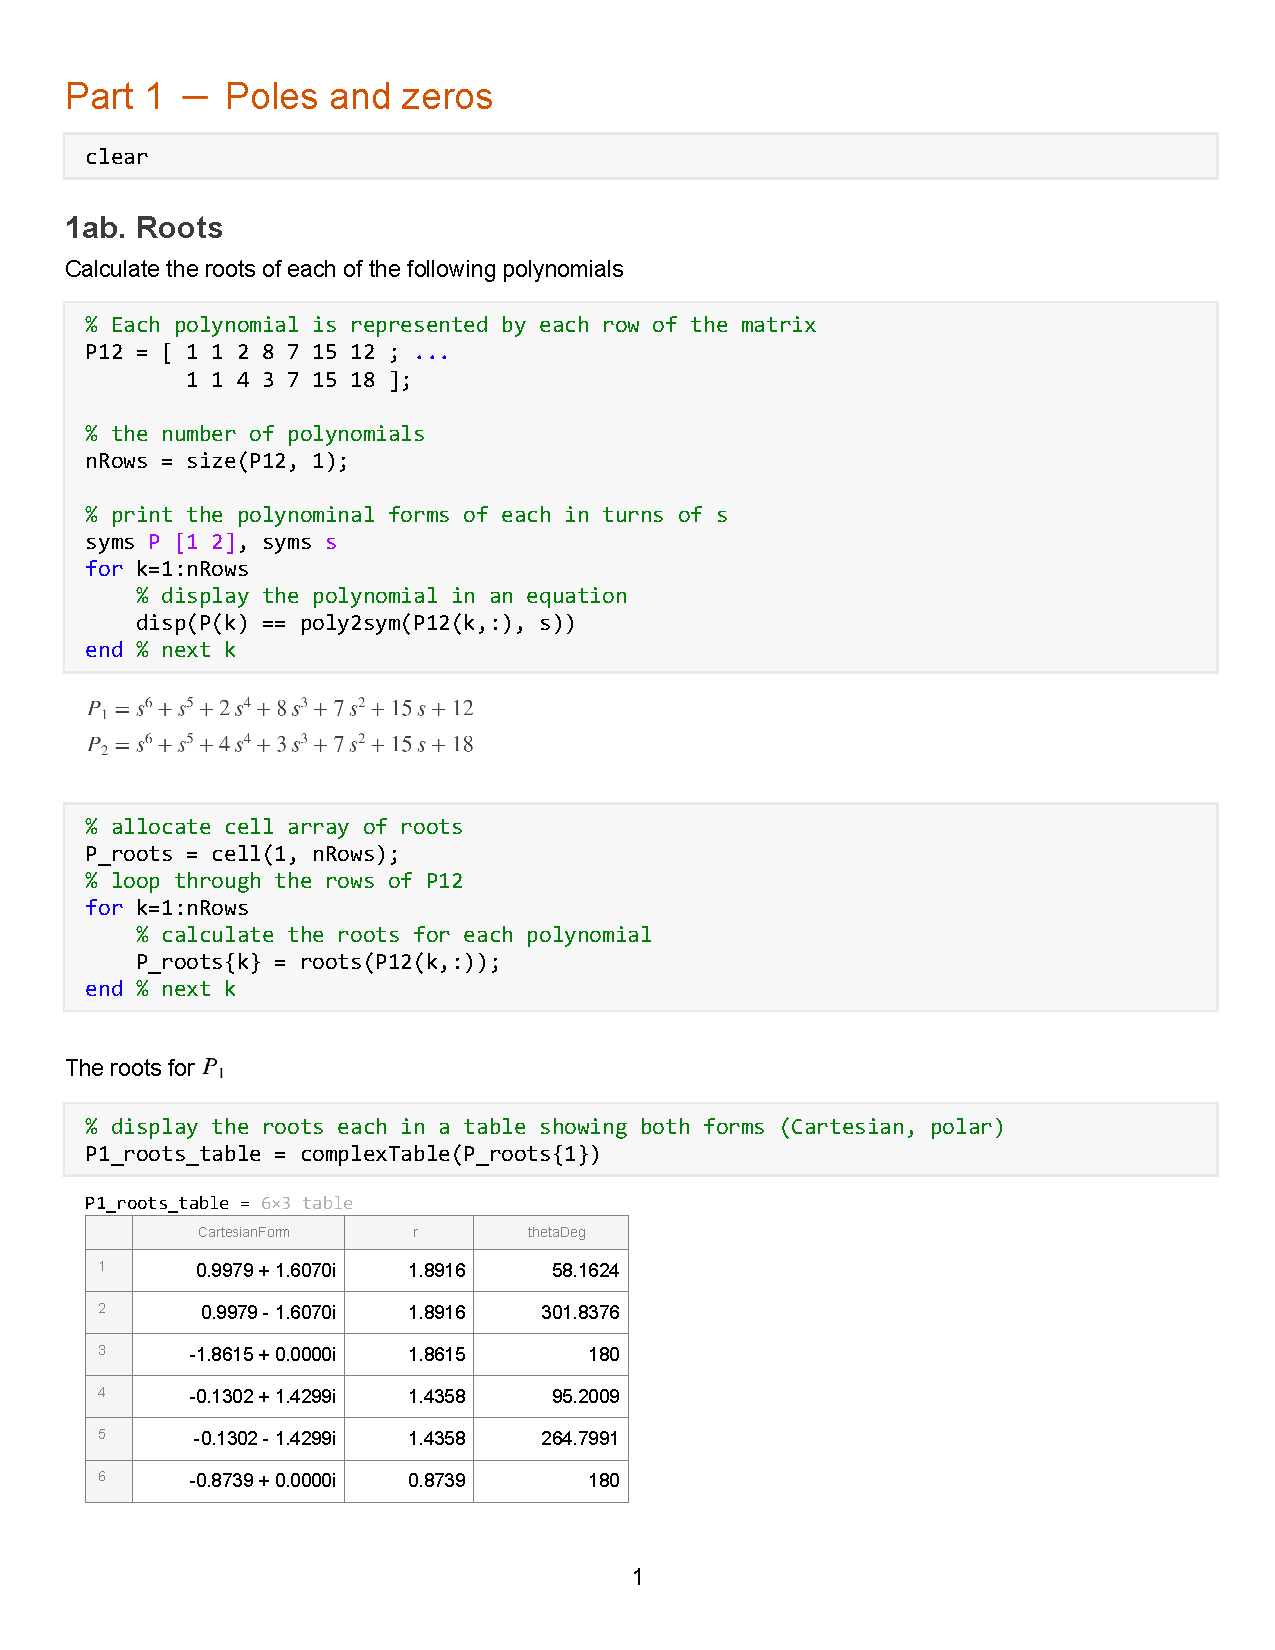
\includepdf[pages={-}]{part01_poles_zeros_mlx.pdf}

\section{Part 2 -- Laplace transforms, Matlab Live Script}

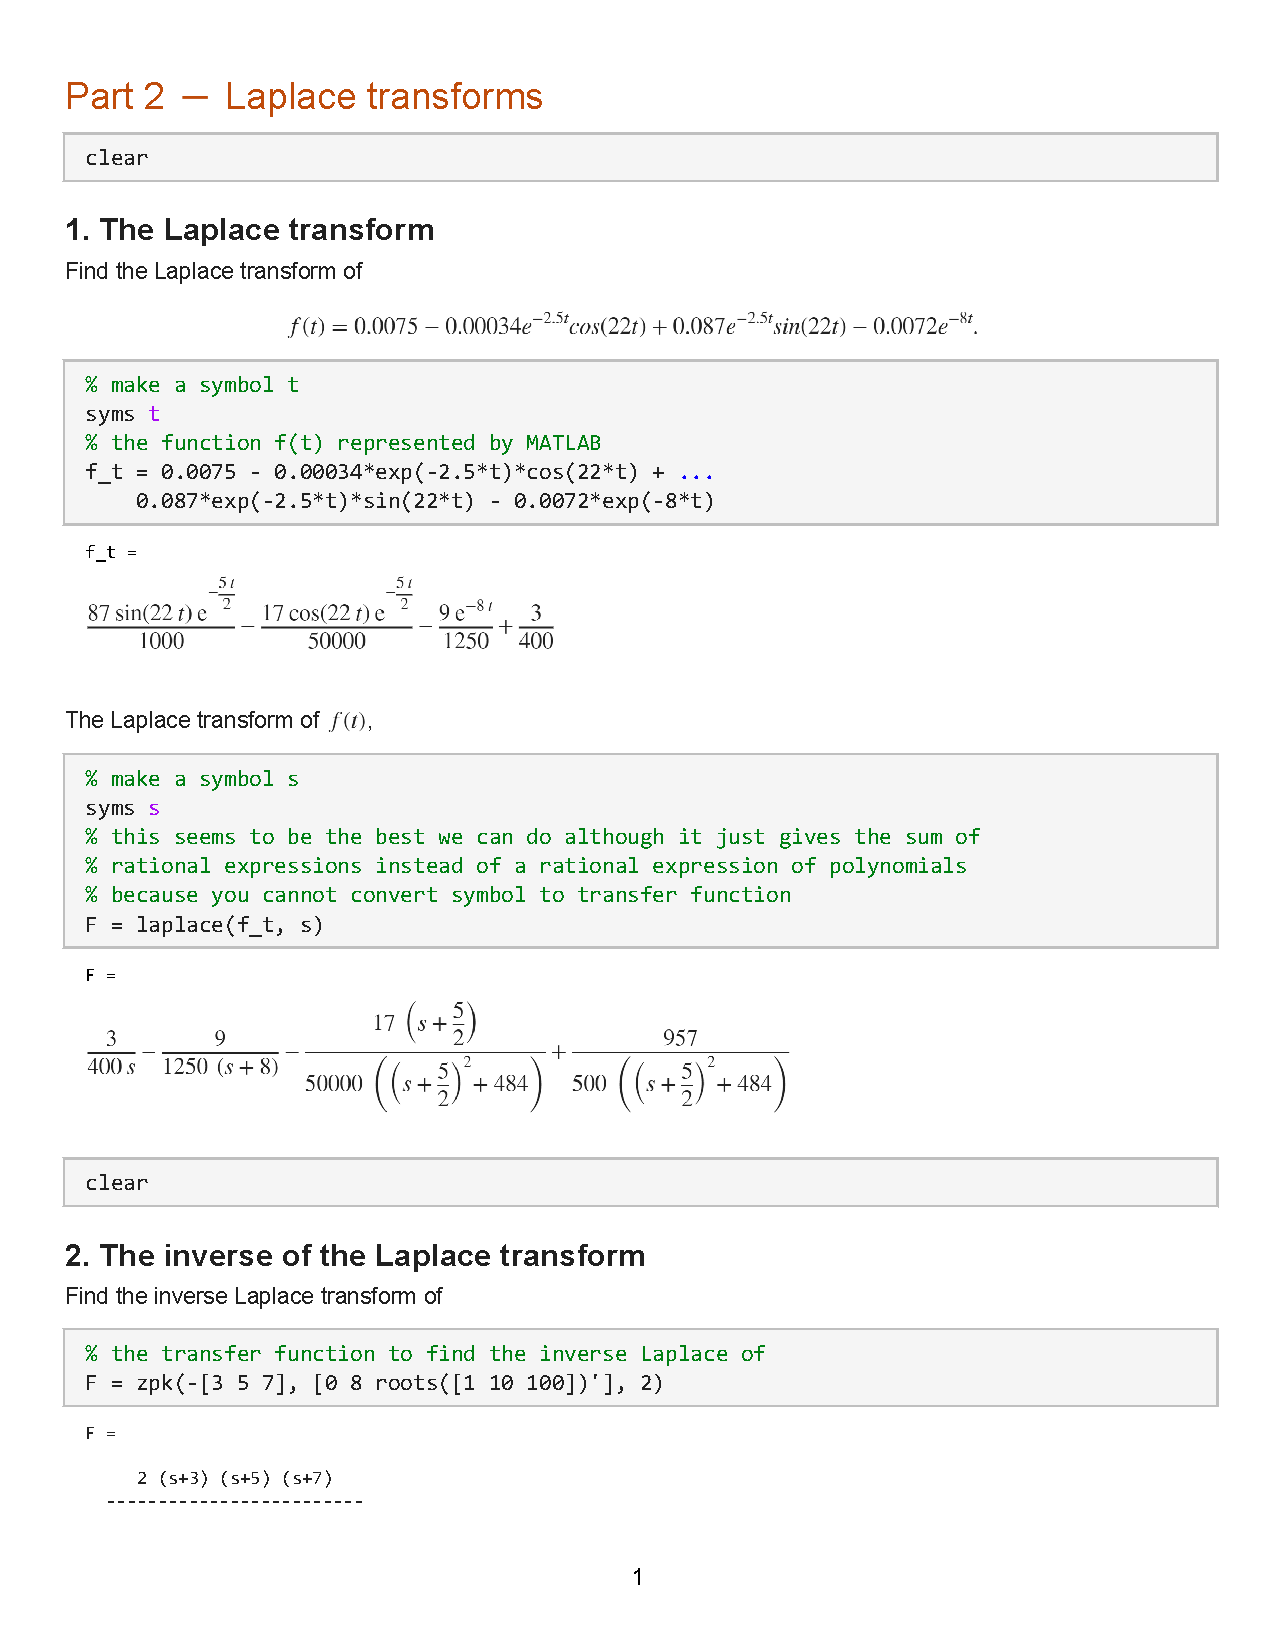
\includepdf[pages={-}]{part02_laplace_transforms_mlx.pdf}

\end{document}
